
\section{T\'ecnicas de conteo}

Muchos problemas de combinatoria implican conteo. Ya que el número de objetos a
contar podría ser muy grande, es importante ser capaz de conta el conjunto de
objetos sin tener que enlistarlos a todos.
% ARREGLAR SALTOS DE PÁGINA
% EIGENVALORES
% VALORES PROPIOS
\subsection{Principio de multiplicaci\'on}

El principio de multiplicación lo utilizamos para contar el número de formas en
las que pueden ocurrir dos eventos simultáneos. El principio de la multiplicación
establece que si un evento puede ocurrir de $n_1$ formas diferentes, y para cada
una de estas ppuede ocurrir un segundo evento simultáneo en $n_2$ formas
diferentes, entonces los dos eventos pueden ocurrir de $n_1 * n_2$ formas
diferentes.

Así, para una serie de $k$ eventos, tenemos:
\begin{theorem}{Principio de multiplicación}{multiplicación}
	\begin{equation}
		n_1*n_2*n_3*...*n_k
		\label{eq:reglaMultiplicacion}
	\end{equation}
\end{theorem}


\subsection{Diagrama de Árbol}

Los diagramas de árbol muestran todos los resultados posibles de un evento. Cada
rama en un diagrama de árbol representa un posible resultado.
Los diagramas de \'arbol pueden usarse para encontrar el n\'umero de resultados
posibles y calcular la probabilidad de los posibles resultados.

%Por ejemplo,

\begin{figure}[h]
	\begin{center}		
	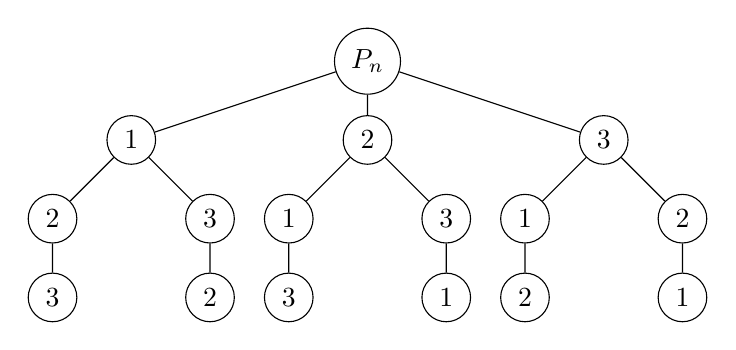
\begin{tikzpicture}[level distance=1cm, level 1/.style={sibling distance=3cm},
		level 2/.style={sibling distance=2cm}, every node/.style={circle, draw,
		align=center} ]
				\centering
				\node[circle,draw]{$P_n$}
		child{node{1} child{node{2} child{node{3}} } child{node{3} child{node{2}}} }
		child{node{2} child{node{1} child{node{3}} } child{node{3} child{node{1}}} }
		child{node{3} child{node{1} child{node{2}} } child{node{2} child{node{1}}} };
			\end{tikzpicture}
		\end{center}
		\caption{Permutaciones para 3 elementos}
		\label{permutaciones_tree}
\end{figure}


\subsection{Principio de adición}

Supongamos que existen $k$ conjuntos de elementos con $n_1$ elementos en el
primer conjunto, $n_2$ elementos en el segundo conjuntos, etc. Si todos los
elementos son distintos, es decir, si si todos los pares dek conjunto $k$ son
disjuntos, entonces el número de elementos de la unión de los conjuntos es $n_1
+ n_2 + ... + n_k $.

Usando la nomenclatura de conjuntos, el principio de adición está definido de la
siguiente manera:

\begin{theorem}{Principio de adición}{adicion}
Sean $A$ y $B$ dos eventos disjuntos, entonces la probabilidad de la unión de
los conjuntos está dada por:

\begin{equation}
	P(A \cup B) = P(A) + P(B)
\end{equation}

De manera general, si el espacio de muestreo tiene un número infinito de
elementos y $A_1, A_2, ... $ son una secuencia de eventos disjuntos, entonces la
probabilidad de la unión es:

\begin{equation}
	P(A_1 \cup A_2 \cup ...) = P(A_1) + P(A_2) + ...
\end{equation}

\end{theorem}


\subsection{Principio del palomar o Principio de Dirichlet}

El principio del palomar, también llamado principio de Dirichlet o principio de
las cajas, establece que si $n$ palomas se distribuyen en $m$ palomares, y si $n
> m$, entonces al menos habrá un palomar con más de una paloma. Otra forma de
decirlo es que $m$ huecos pueden albergar como mucho $m$ objetos si cada uno de
los objetos está en un hueco distinto, así que el hecho de añadir otro objeto
fuerza a volver a utilizar alguno de los huecos, como se observa en la Fig.
(\ref{palomar}). A manera de ejemplo: si se toman trece personas, al menos dos
habrán nacido el mismo mes.

\begin{figure}[h]
	\centering
	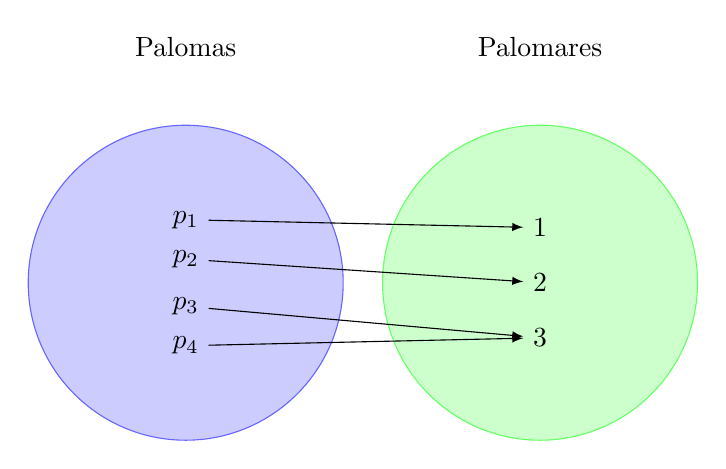
\begin{tikzpicture}
		% draw the sets
		\filldraw[fill=blue!20, draw=blue!60] (-1.5,0) circle (2cm);
		\filldraw[fill=green!20, draw=green!60] (3,0) circle (2cm);
	
	
		% the texts
		\node at (-1.5,3) {Palomas};
		\node at (3,3) {Palomares};
	
		% the circles and the arrows
		\node (x1) at (-1.5,0.8) {$p_1$};
		\node (x2) at (-1.5,0.3) {$p_2$};
		\node (x3) at (-1.5,-0.3) {$p_3$};
		\node (x4) at (-1.5,-0.8) {$p_4$};
		
		\node (y1) at (3,0.7) {$1$};
		\node (y2) at (3,0) {$2$};
		\node (y3) at (3,-0.7) {$3$};
	
		% draw the arrows
		\draw[-latex] (x1) -- (y1);
		\draw[-latex] (x2) -- (y2);
		\draw[-latex] (x3) -- (y3);
		\draw[-latex] (x4) -- (y3);
	
	\end{tikzpicture}
\caption{Ilustración del principio del palomar. El conjunto de las palomas es
mayor al del palomar, por lo tanto en al menos un palomar deben de haber dos
palomas.}
\label{palomar}
	\end{figure}




\subsection{Permutaciones}

\begin{tcolorbox}[colback=gray!5!white,colframe=gray!60!black,title=Definición: Permutación]
	Una \textbf{permutaci\'on} de un conjunto es un arreglo u ordenamiento de sus
	elementos sin repeticiones ni omisiones.
	
	Si el conjunto está ordenado, el proceso de reordenar sus elementos, es una permutación.
	\label{Permutaciones_definition}
\end{tcolorbox}

Para saber el n\'umero de permutaciones que existen de un conjunto se debe
conocer su cardinalidad. Tomemos como ejemplo, el conjunto de n\'umeros enteros
$A=\{1, 2, 3\}$. Para cualquier permutaci\'on, en la primera posici\'on pueden
colocarse cualquiera de los tres elementos; en la segunda posición se pueden
colocar dos posibles elementos; mientras que al final, se puede colocar una
posibilidad.

En general, para cualquier conjunto de elementos $X$ de cardinalidad $|n|$, en
la primera posici\'on se pueden colocar $n$ elementos, para la siguiente
posici\'on $n-1$. Así sucesivamente hasta las \'ultimas posiciones, donde se
pueden colocar $3, 2$ y $1$ elementos. De esta manera, se dice que el n\'umero
de permutaciones es:

\begin{theorem}{Permutación}{permutacion}
	\begin{equation}
		P_n=n*(n-1)*(n-2)*...*3*2*1=n!
		\label{permutaciones_totales}
	\end{equation}
	
	Remarcando el hecho de que $0! = 1$.

\end{theorem}

\subsubsection{Permutaciones de $k$-elementos}

Sea un conjunto de elementos $X$ de cardinalidad $|n|$, como en el caso
anterior. Supongamos que deseamos tomar $k$ elementos del conjunto y contar las
diferentes formas en las que podríamos agarrarlos.

De primera instancia, podemos tomar cualquiera de los $n$ objetos como el primer
elemento. Posteriormente, solo hay $n-1$ elementos para la segunda opción y asi
sucesivamente hasta que llegamos al $k$-ésimo elemento. Lo que nos deja
$n-(k-1)$ opciones para la última opción.

Podemos partir de la Ec. (\ref{permutaciones_totales}) para hacer la permutación
de los $n$ elementos, sin embargo, tendríamos que ajustar la fórmula para que
escojamos solo $k$ de los $n$ elementos ($n-k$).
\begin{equation}
n(n-1)(n-2)...(n-(k-1))\overbrace{(n-k)(n-(k+1))...1}^{(n-k)!}
\end{equation}

Para quitar los elementos repetidos, dividimos la ecuación anterior entre el
número de elementos repetidos, de la siguiente manera:

\begin{equation}
 = \frac{ n (n-1) (n-2) ... (n-k+1) \overbrace{(n-k)(n-(k+1))...1}^{(n-k)!}}{\underbrace{(n-k)(n-k-1) ... 1}_{(n-k)!}}
\end{equation}

Lo que nos lleva a la Ec. (\ref{k-permutaciones}).

\begin{theorem}{Permutación}{permutacion}
El total de permutaciones de $n$ objetos distintos tomados de $k$ formas a la
vez, está dado por:

	\begin{equation}
		P(n,r) = \frac{n!}{(n-k)!}
		\label{k-permutaciones}
	\end{equation}
\end{theorem}


\subsubsection{Paridad de una permutación}

En una permutación, ocurre una \textbf{inversi\'on} cuando un elemento mayor
precede a un elemento menor. Para conocer el n\'umero de inversiones se siguen
los siguientes pasos:

\begin{itemize}
\item Tomar el primer elemento de la permutaci\'on
\item Contar los enteros menores a la derecha del elemento en cuesti\'on
\item Realizar los dos pasos anteriores para cada elemento de la permutaci\'on
\item Sumar el total de inversiones contadas para cada elemento
\end{itemize}

\textbf{Ejemplo}:

Se toma la permutación \textbf{$A=\{6,1,3,4,5,2\}$}\\

Primer elemento: $6$; menores a la derecha: $1,3,4,5,2$; n\'umero de
inversiones: \textbf{5}
Primer elemento: $1$; menores a la derecha: $\emptyset$; n\'umero de
inversiones: \textbf{0}
Primer elemento: $3$; menores a la derecha: $2$; n\'umero de inversiones:
\textbf{1}\\
Primer elemento: $4$; menores a la derecha: $2$; n\'umero de inversiones:
\textbf{1}\\
Primer elemento: $5$; menores a la derecha: $2$; n\'umero de inversiones:
\textbf{1}\\

Total de inversiones: \textbf{8}
\begin{tcolorbox}[colback=gray!5!white,colframe=gray!60!black,title=Definición: Tipos de permutaciones]
	\textbf{Permutaci\'on par:} aquella en la que el total de inversiones es un
	entero par.
	
	\tcblower

	\textbf{Permutaci\'on impar}: aquella en la que el total de inversiones es un
	entero impar.
	
\end{tcolorbox}


\subsection{Combinación}

\subsection{El problema de Monty Hall}

El problema de \textit{Monty Hall} o paradoja del presentador es un problema de
probailidad condicional basado en el concurso de televisi\'on estadounidense
\textit{Let's Make a Deal}. El problema fue bautizado as\'i por el nombre del
presentador de dicho programa.

En 1975, el matem\'atico Steve Selvin resuelve este problema y es publicado en
la revista \textit{American Statistician}. Posteriormente fue popularizado por
Marilyn vos Savant en la revista \textit{Parade Magazine}, en 1990. El problema
dice as\'i:

\textbf{Planteamiento del problema:}

Hay tres puertas. Detr\'as de una de ellas, hay un premio. Detr\'as de cada una
de las dos puertas restantes hay una cabra.

Cada puerta tiene la misma probabilidad de contener el premio.

Se te da a seleccionar una de las tres puertas como una oportunidad de ganar el
premio. Sin embargo, una vez que se ha seleccionado la puerta, el presentador
destapa una de ellas y te muestra que detrás hab\'ia una cabra.Una vez dada esa
informaci\'on, el presentador te pregunta si deseas cambiar de puerta o
conservar tu elecci\'on.

La pregunta crucial es:

Dado que el presentador ha destapado una puerta y mostrado que no estaba el
premio, ¿es m\'as conveniente cambiar mi opci\'on o conservar mi elecci\'on de
la puerta inicial?

%\begin{figure}[h]
%	\centering
%	\includegraphics[scale=0.5]{Images/Monty Hall}
%	\caption{Imagen ilustratuiva del problema de Monty Hall}
%\end{figure}

\subsection{Soluci\'on:}
Este problema es un ejercicios relativamente simple de probabilidad condicional.
Sin embargo, se debe tener cuidado, pues es un problema particularmente confuso.
Se abrodará desde dos enfoques.

Dos observaciones son cruciales para entender el problema:

\begin{itemize}
\item El presentador conoce la puerta donde se encuentra el premio y obviamente
no revelará esa puerta. 
\item Monty revelar\'a cualquiera de las otras dos puertas de forma aleatoria y
con con igual probabilidad de que esto ocurra.
\end{itemize}
Supongase que selecciona la puerta 1. Entonces pueden ocurrir tres casos:
\begin{enumerate}
\item El premio está en la puerta 1. Monty abre la puerta 2 o la 3. Si se cambia
la elecci\'on, se pierde. Si se conserva la elecci\'on, ganas.
\item El premio está en la puerta 2. Monty abre la puerta 3. Si se cambia de
elecci\'on, se gana. Si se conserva la elecci\'on, pierdes.
\item El premio está en la pierta 3. Monty abre la puerta 2. Si se cambia de
elecci\'on, se gana. Si se conserva la elecci\'on, pierdes.
\end{enumerate}
Se debe notar que al cambiar de elecci\'on se gana en 2 de los 3 casos; mientras
que al conservar la elecci\'on, se gana s\'olo en 1 de los 3 casos. Por lo
tanto, la probabilidad de ganar si se cambia de puerta, es de $\frac{2}{3}$. Por
otro lado, la probabilidad de ganar con la elecci\'on inicial es de
$\frac{1}{3}$.

Conclusi\'on: ¡Cambia de puerta!



\subsection{Problema del cumpleaños}

Este problema se presenta a menudo como ejemplo en el c\'alculo de
probabilidades Ec. (\ref{eq:probabilidad}). Este problema puede ser enunciado de la siguiente
forma. 

\textit{En un grupo de $n$ personas escogidas al azar, ¿cuál es la probabilidad de que
al menos dos de ellas tengan el mismo d\'ia de cumpleaños?}

Se asume que los nacimientos se distribuyen de manera uniforme a lo largo de
todo el año, y, por simplicidad, también asumimos que no existe el 29 de
febrero.

Otra forma alternativa de presentar el problema es la siguiente:

\textit{¿Cuál es el número mínimo de personas necesario en un grupo para que sea más
probable encontrar al menos dos con el mismo d\'ia de cumpleaños?}

Resolveremos la primera versión del problema, ya que con esto podremos hallar
también la respuesta a la segunda versión.

Soluci\'on.

Comenzaremos por resolver el problema para un tamaño muestral $n = 1, 2$ y $3$,
y posteriormente extenderemos el razonamiento al caso general. Para $n = 1$ , es
decir, cuando s\'olo hay una persona, la probabilidad $P_1$ de coincidir con otra
persona es cero, dado que no existe otra persona. Para $n = 2$, esto es, hay dos
personas, la probabilidad $P_2$ de que coincidan en su d\'ia de cumpleaños de
acuerdo con la Ec. (\ref{eq:probabilidad}) es:


\begin{equation}
P_2 = \frac{365}{365^2} = \frac{1}{365}
\end{equation}

ya que hay 365 maneras diferentes de que su día de cumpleaños coincida
(una por cada día del año), y $365 \cdot 365 = 3652$ maneras diferentes de que
se produzcan sus cumpleaños.

Para $n = 3$ personas, podemos calcular la probabilidad $p_3$ de que al menos
dos de ellas coincidan en su día de cumpleaños, a partir de la Ec.
(\ref{eq:complementRule}), como 1 menos la probabilidad del suceso contrario, es
decir, menos la probabilidad de que todas ellas cumplan años en d\'ias
diferentes.

De esta forma, tenemos:

\begin{equation}
p_3 = 1- \frac{364}{365} = 1 - \frac {364 \cdot 363}{365^2}
\end{equation}

%ya que la segunda persona puede cumplir años en cualquiera de los 365 días del
%año, pero s\'olo en 364 de ellos \'este no coincidirá con el cumpleaños de la
%primera persona; de igual forma, el cumpleaños de la tercera persona no
%coincidir\'a con el cumpleaños de las otras dos en 363 de los 365 casos
%posibles. Aplicando el mismo razonamiento para cualquier $n$ entre 1 y 365,
%obtenemos:
%
%\begin{equation}
%	\begin{array}{l}
%		P_n = 1 - \frac{364}{365} \cdot \frac{364}{365} \cdot \frac{364}{365} ...
%	
%			= 1 - \frac{365 \cdot - n + 1}{365} \\
%	
%			= \frac {364 \cdot 362 \cdot 363 \cdot 362 ... ( 365-n+1)}
%				{365^{n-1}} \\
%	
%			= \frac {364 \cdot 362 \cdot 363 \cdot 362 ... (365-n+1)}
%				{365^{n}} \\
%	
%			= \frac{365!} {365^n \cdot (365-n)!}
%
%	\end{array}
%\end{equation}
%
%Con lo que damos soluci\'on al problema 1. Obviamente, $P_n$ es 1 para todo $n$
%mayor que 365 (en una reuni\'on de más de 365 personas, necesariamente ha de
%haber al menos dos personas con el mismo d\'ia de cumpleaños). En el cuadro 1
%mostramos los valores que toma la probabilidad $p_n$ para algunos valores de n,
%seg\'un la expresi\'on (\ref{e6}) que acabamos de calcular.
%




\subsection{Resumen de técnicas de conteo}

\begin{tcolorbox}[colback=blue!5!white,colframe=blue!60!black,title=Resumen: Técnicas de conteo]

	\begin{itemize}
		\item \textbf{Permutaciones} de $n$ objetos:
		\begin{center}
		$n!$
		\end{center}

		\item \textbf{\textit{k}-Permutaciones} de $n$ objetos:
		\begin{center}
		$\frac{n!}{(n-k)!}$
		\end{center}

		\item \textbf{Combinaciones} de $k$ de $n$ objetos:
		\begin{center}
		$\binom{n}{k} = \frac{n!}{k!(n-k)!}$
		\end{center}

		\item \textbf{Particiones} de $n$ objetos en $r$ grupos, con el \textit{i}-ésimo
		grupo con $n_i$ objetos:
		\begin{center}
			$\binom{n}{n_1,n_2,...,n_r} = \frac{n!}{n_1!,n_2!,...,n_r!}$
		\end{center}

	\end{itemize}
	
\end{tcolorbox}
